\documentclass{standalone}
\usepackage{tikz}
\usetikzlibrary{patterns}
\usetikzlibrary{positioning}
\usetikzlibrary{patterns, positioning}
\usetikzlibrary{shapes.misc}
\usepackage[outline]{contour}
\contourlength{1.5pt} 
\usepackage[sfdefault]{ClearSans}

\begin{document}
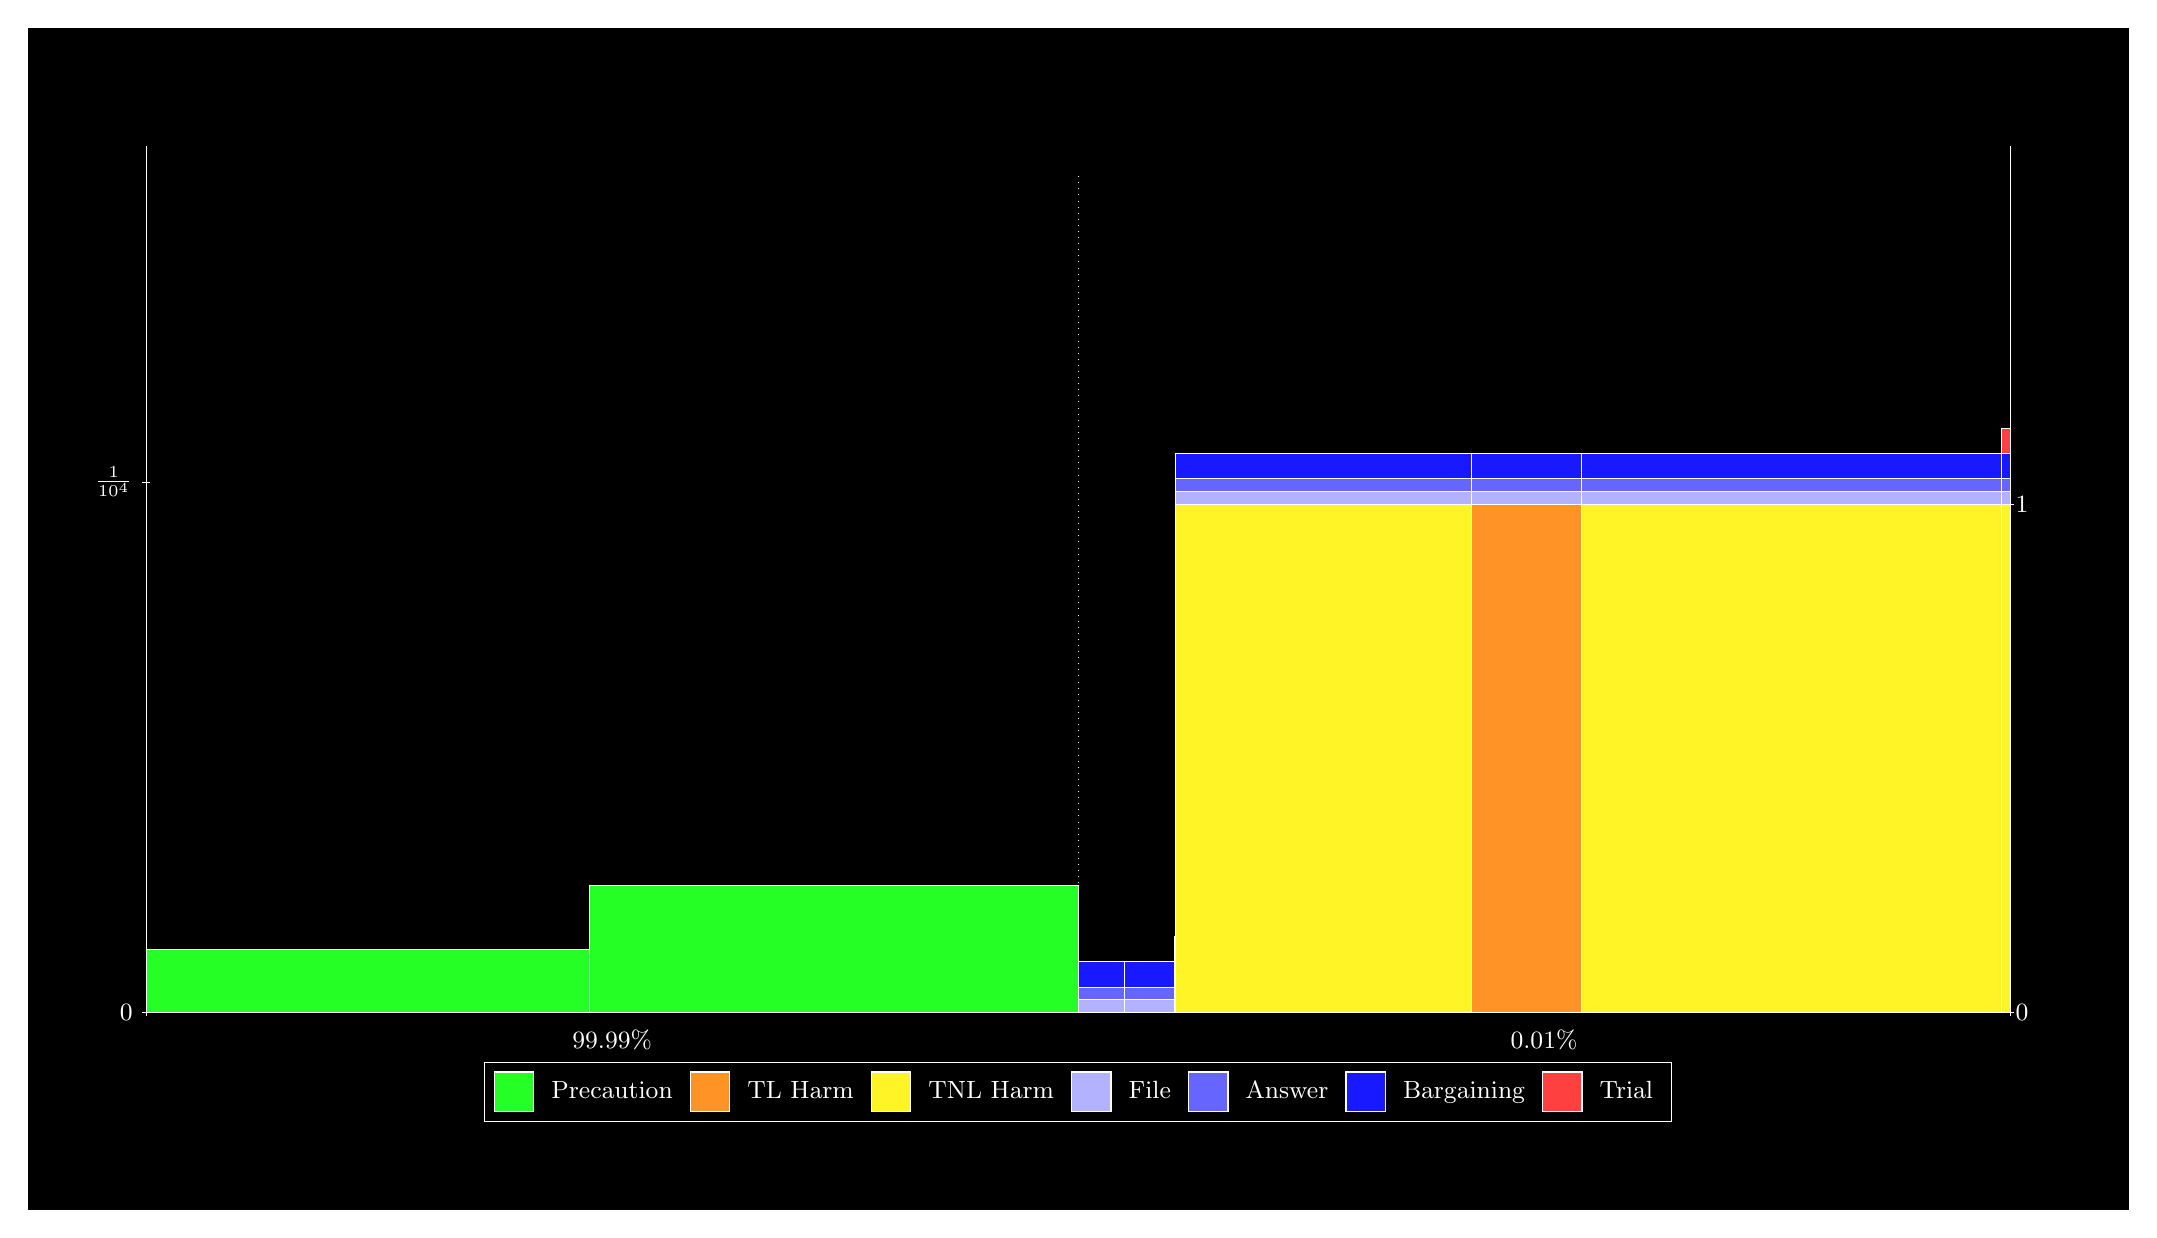
\begin{tikzpicture}
\draw[fill=black] (0,0) rectangle (26.667,15);
\draw[fill=green!85,draw=white,very thin] (1.5,2.5) rectangle (7.1207,3.3087);
\draw[fill=green!85,draw=white,very thin] (7.1207,2.5) rectangle (13.333,4.1173);
\draw[fill=green!85,draw=white,very thin] (13.333,2.5) rectangle (13.92,2.5001);
\draw[fill=blue!30,draw=white,very thin] (13.333,2.5001) rectangle (13.92,2.6615);
\draw[fill=blue!60,draw=white,very thin] (13.333,2.6615) rectangle (13.92,2.8229);
\draw[fill=blue!90,draw=white,very thin] (13.333,2.8229) rectangle (13.92,3.1457);
\draw[fill=green!85,draw=white,very thin] (13.92,2.5) rectangle (14.553,2.5002);
\draw[fill=blue!30,draw=white,very thin] (13.92,2.5002) rectangle (14.553,2.6616);
\draw[fill=blue!60,draw=white,very thin] (13.92,2.6616) rectangle (14.553,2.823);
\draw[fill=blue!90,draw=white,very thin] (13.92,2.823) rectangle (14.553,3.1458);
\draw[fill=green!85,draw=white,very thin] (14.553,2.5) rectangle (14.568,2.5002);
\draw[fill=blue!30,draw=white,very thin] (14.553,2.5002) rectangle (14.568,2.6616);
\draw[fill=blue!60,draw=white,very thin] (14.553,2.6616) rectangle (14.568,2.823);
\draw[fill=blue!90,draw=white,very thin] (14.553,2.823) rectangle (14.568,3.1458);
\draw[fill=red!75,draw=white,very thin] (14.553,3.1458) rectangle (14.568,3.4686);
\draw[fill=green!85,draw=white,very thin] (14.568,2.5) rectangle (18.323,2.5001);
\draw[fill=yellow!85,draw=white,very thin] (14.568,2.5001) rectangle (18.323,8.9567);
\draw[fill=blue!30,draw=white,very thin] (14.568,8.9567) rectangle (18.323,9.1181);
\draw[fill=blue!60,draw=white,very thin] (14.568,9.1181) rectangle (18.323,9.2795);
\draw[fill=blue!90,draw=white,very thin] (14.568,9.2795) rectangle (18.323,9.6023);
\draw[fill=green!85,draw=white,very thin] (18.323,2.5) rectangle (19.727,2.5001);
\draw[fill=orange!85,draw=white,very thin] (18.323,2.5001) rectangle (19.727,8.9567);
\draw[fill=blue!30,draw=white,very thin] (18.323,8.9567) rectangle (19.727,9.1181);
\draw[fill=blue!60,draw=white,very thin] (18.323,9.1181) rectangle (19.727,9.2795);
\draw[fill=blue!90,draw=white,very thin] (18.323,9.2795) rectangle (19.727,9.6023);
\draw[fill=green!85,draw=white,very thin] (19.727,2.5) rectangle (25.053,2.5002);
\draw[fill=yellow!85,draw=white,very thin] (19.727,2.5002) rectangle (25.053,8.9568);
\draw[fill=blue!30,draw=white,very thin] (19.727,8.9568) rectangle (25.053,9.1182);
\draw[fill=blue!60,draw=white,very thin] (19.727,9.1182) rectangle (25.053,9.2796);
\draw[fill=blue!90,draw=white,very thin] (19.727,9.2796) rectangle (25.053,9.6024);
\draw[fill=green!85,draw=white,very thin] (25.053,2.5) rectangle (25.167,2.5002);
\draw[fill=yellow!85,draw=white,very thin] (25.053,2.5002) rectangle (25.167,8.9568);
\draw[fill=blue!30,draw=white,very thin] (25.053,8.9568) rectangle (25.167,9.1182);
\draw[fill=blue!60,draw=white,very thin] (25.053,9.1182) rectangle (25.167,9.2796);
\draw[fill=blue!90,draw=white,very thin] (25.053,9.2796) rectangle (25.167,9.6024);
\draw[fill=red!75,draw=white,very thin] (25.053,9.6024) rectangle (25.167,9.9252);
\draw[white,very thin] (1.5,2.5) -- (1.5,13.5);
\draw[white,very thin] (1.45,2.5) -- (1.55,2.5);
\node[font=\small,text=white, anchor=east] at (1.45, 2.5) {0};
\draw[white,very thin] (1.45,9.2388) -- (1.55,9.2388);
\node[font=\small,text=white, anchor=east] at (1.45, 9.2388) {$\frac{1}{10^{4}}$};

\draw[white,dotted,very thin] (13.333,2.83) -- (13.333,13.17);
\draw[white,very thin] (25.167,2.5) -- (25.167,13.5);
\draw[white,very thin] (25.117,2.5) -- (25.217,2.5);
\node[font=\small,text=white, anchor=west] at (25.117, 2.5) {0};
\draw[white,very thin] (25.117,8.9566) -- (25.217,8.9566);
\node[font=\small,text=white, anchor=west] at (25.117, 8.9566) {1};

\draw[white,very thin] (1.5,2.5) -- (25.167,2.5);
\draw[white,very thin] (1.5,2.45) -- (1.5,2.55);
\node[font=\small,text=white, anchor=north] at (1.5, 2.45) {};
\draw[white,very thin] (25.167,2.45) -- (25.167,2.55);
\node[font=\small,text=white, anchor=north] at (25.167, 2.45) {};

\node[font=\small,text=white,anchor=south] at (7.4167, 1.9) {99.99\%};
\node[font=\small,text=white,anchor=south] at (19.25, 1.9) {0.01\%};
\draw (13.3333,2.5) node (B) {};
\begin{scope}[align=center]
\matrix[scale=0.5,draw=white,below=0.5cm of B,nodes={draw},column sep=0.1cm]{
\node[rectangle,draw,minimum width=0.5cm,minimum height=0.5cm,fill=green!85]{}; & \node[draw=none,font=\small,text=white]{Precaution}; &
\node[rectangle,draw,minimum width=0.5cm,minimum height=0.5cm,fill=orange!85]{}; & \node[draw=none,font=\small,text=white]{TL Harm}; &
\node[rectangle,draw,minimum width=0.5cm,minimum height=0.5cm,fill=yellow!85]{}; & \node[draw=none,font=\small,text=white]{TNL Harm}; &
\node[rectangle,draw,minimum width=0.5cm,minimum height=0.5cm,fill=blue!30]{}; & \node[draw=none,font=\small,text=white]{File}; &
\node[rectangle,draw,minimum width=0.5cm,minimum height=0.5cm,fill=blue!60]{}; & \node[draw=none,font=\small,text=white]{Answer}; &
\node[rectangle,draw,minimum width=0.5cm,minimum height=0.5cm,fill=blue!90]{}; & \node[draw=none,font=\small,text=white]{Bargaining}; &
\node[rectangle,draw,minimum width=0.5cm,minimum height=0.5cm,fill=red!75]{}; & \node[draw=none,font=\small,text=white]{Trial}; \\\\
};\end{scope}

\end{tikzpicture}
\end{document}